\documentclass[tikz,border=5pt]{standalone}
\usepackage{amsmath,amssymb}
\usepackage{amsfonts}

\usetikzlibrary{arrows.meta, positioning, calc}

\begin{document}
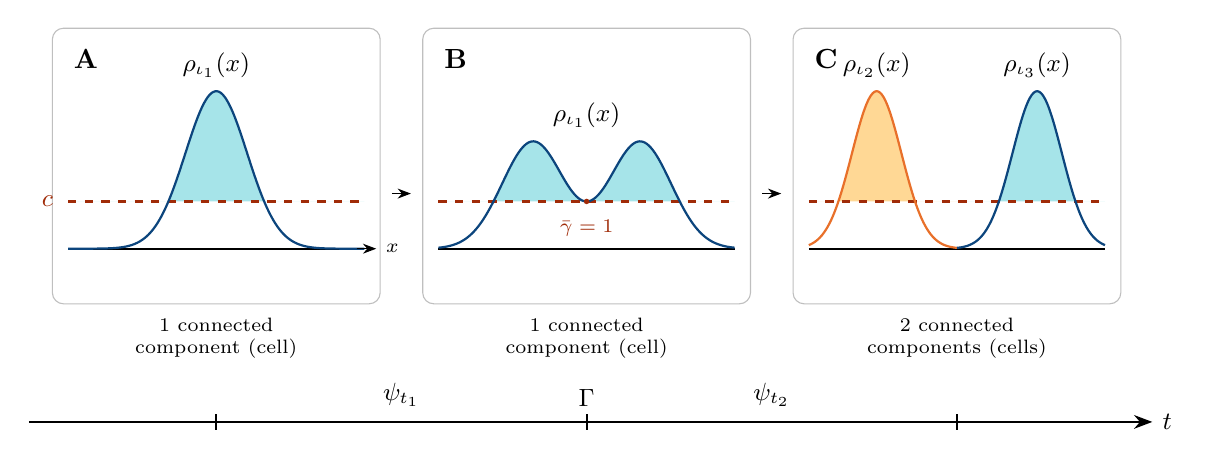
\begin{tikzpicture}[
    every node/.style={font=\small},
    axisline/.style={thick, colorAxis},
    curve/.style={thick, colorCurve, smooth},
    curveA/.style={thick, colorCurveA, smooth},
    curveB/.style={thick, colorCurveB, smooth},
    threshold/.style={thick, dashed, colorThreshold},
]

    % ---------------------------------------------------------------------------
    % Global color palette for this figure.
    % Axes/frames/text use black; data colors are taken from the 6-color
    % palette defined in figures/abm-theory/simple_abm.py (COLOR1--COLOR6).
    % Change these definitions to re-theme the whole figure at once.
    % ---------------------------------------------------------------------------
    \definecolor{colorAxis}{HTML}{000000}          % black -- axes, ticks, frames, text
    \definecolor{colorThreshold}{HTML}{A02B08}     % simple_abm.py COLOR6
    \definecolor{colorCurve}{HTML}{0C457D}         % simple_abm.py COLOR3
    \definecolor{colorFillMerged}{HTML}{6BD2DB}    % simple_abm.py COLOR1
    \definecolor{colorCurveA}{HTML}{0C457D}        % simple_abm.py COLOR3
    \definecolor{colorFillDaughterA}{HTML}{6BD2DB} % simple_abm.py COLOR1
    \definecolor{colorCurveB}{HTML}{E8702A}        % simple_abm.py COLOR5
    \definecolor{colorFillDaughterB}{HTML}{FFBE4F} % simple_abm.py COLOR4
    \colorlet{colorFrame}{colorAxis!25!white}
    \newcommand{\fillOpacity}{0.6}

    % -----------------------------------------------------------------------
    % Shared numeric parameters
    % -----------------------------------------------------------------------
    % \S is the single horizontal scale factor used to fit the whole figure
    % to exactly \textwidth of the thesis (a4paper, inner=3.5cm, outer=2.5cm
    % as set in main-book.tex, i.e. \textwidth = 426.79135pt).
    % All x-related lengths (domain, spacing, sigma/mu of the density
    % functions) are multiplied by \S; since sigma and mu scale together the
    % peak heights and the saddle/threshold relations stay exact.
    \pgfmathsetmacro{\S}{0.78386}
    \def\yScale{2.0}         % vertical amplification of the density values
    \def\cThresh{0.3}        % division/connectivity threshold (unscaled, in [0,1])
    \def\panelShiftY{2.2}    % vertical offset of the panels above the time axis

    \pgfmathsetmacro{\domainMin}{-2.4*\S}
    \pgfmathsetmacro{\domainMax}{2.4*\S}
    \pgfmathsetmacro{\panelSpacing}{6*\S}
    \pgfmathsetmacro{\nSamples}{160}

    % sigma/mu of the underlying Gaussians (unscaled values chosen first,
    % then multiplied by \S so shapes stay identical, only smaller)
    \pgfmathsetmacro{\sigmaOne}{0.5*\S}
    \pgfmathsetmacro{\sigmaTwo}{0.5*\S}
    \pgfmathsetmacro{\muTwo}{0.8693*\S}    % chosen so the saddle exactly touches cThresh (see below)
    \pgfmathsetmacro{\ampTwo}{0.68}
    \pgfmathsetmacro{\sigmaThree}{0.4*\S}
    \pgfmathsetmacro{\muThree}{1.3*\S}

    % Density functions (unscaled amplitude, i.e. in [0,1]-ish units), parametrized by \x
    \newcommand{\rhoOne}[1]{exp(-((#1)^2)/(2*\sigmaOne^2))}
    \newcommand{\rhoTwoMerged}[1]{\ampTwo*(exp(-(((#1)-\muTwo)^2)/(2*\sigmaTwo^2)) + exp(-(((#1)+\muTwo)^2)/(2*\sigmaTwo^2)))}
    \newcommand{\rhoThreeA}[1]{exp(-(((#1)-\muThree)^2)/(2*\sigmaThree^2))}
    \newcommand{\rhoThreeB}[1]{exp(-(((#1)+\muThree)^2)/(2*\sigmaThree^2))}

    % -----------------------------------------------------------------------
    % Time axis
    % -----------------------------------------------------------------------
    \draw[thick, ->, >=Stealth, colorAxis] (\domainMin-0.5,0) -- (2*\panelSpacing+\domainMax+0.6,0) node[right] {$t$};
    \foreach \x in {0,\panelSpacing,2*\panelSpacing} {
        \draw[thick, colorAxis] (\x,0.1) -- (\x,-0.1);
    }
    \node[above=2pt] at (0.5*\panelSpacing,0) {$\psi_{t_1}$};
    \node[above=2pt] at (1.0*\panelSpacing,0) {$\Gamma$};
    \node[above=2pt] at (1.5*\panelSpacing,0) {$\psi_{t_2}$};

    % =========================================================================
    % Panel 1 (t0): single peak -- one cell, one connected component
    % =========================================================================
    \begin{scope}[shift={(0,\panelShiftY)}]
        \draw[rounded corners, colorFrame, thin]
            (\domainMin-0.2,-0.7) rectangle (\domainMax+0.2,\yScale*1.25+0.3);
        \node[anchor=north west, font=\bfseries] at (\domainMin-0.05,\yScale*1.25+0.15) {A};

        % superlevel-set fill: top boundary follows max(rho,cThresh), so the
        % shaded region only bulges above the baseline where rho exceeds the
        % threshold -- this is exactly the superlevel set {x : rho(x) >= c}
        \fill[colorFillMerged, opacity=\fillOpacity]
            plot[domain=\domainMin:\domainMax, samples=\nSamples]
                (\x,{\yScale*max(\rhoOne{\x},\cThresh)})
            -- (\domainMax,{\yScale*\cThresh}) -- (\domainMin,{\yScale*\cThresh}) -- cycle;

        \draw[axisline] (\domainMin,0) -- (\domainMax,0);
        \draw[threshold] (\domainMin,{\yScale*\cThresh}) -- (\domainMax,{\yScale*\cThresh});
        \node[left=2pt, colorThreshold] at (\domainMin,{\yScale*\cThresh}) {$c$};

        \draw[curve] plot[domain=\domainMin:\domainMax, samples=\nSamples] (\x,{\yScale*\rhoOne{\x}});

        \node[above] at (0,{\yScale*1.0+0.05}) {$\rho_{\iota_1}(x)$};
        \node[below=10pt, font=\scriptsize, align=center] at (0,-0.4) {1 connected\\component (cell)};

        \draw[->, >=Stealth, thin, colorAxis] (\domainMax-0.1,0) -- (\domainMax+0.15,0) node[right, font=\scriptsize] {$x$};
    \end{scope}

    % =========================================================================
    % Panel 2 (t1): two peaks emerging -- the saddle between them is
    % constructed to touch the threshold exactly, marking the singular
    % instant at which the division criterion becomes active
    % ($\bar\gamma=1$, cf. the two overlapping circles touching in exactly
    % one point). Up to and including this instant the superlevel set is
    % still a single connected component, i.e. still one identifier $\iota_1$.
    % =========================================================================
    \begin{scope}[shift={(\panelSpacing,\panelShiftY)}]
        \draw[rounded corners, colorFrame, thin]
            (\domainMin-0.2,-0.7) rectangle (\domainMax+0.2,\yScale*1.25+0.3);
        \node[anchor=north west, font=\bfseries] at (\domainMin-0.05,\yScale*1.25+0.15) {B};

        \fill[colorFillMerged, opacity=\fillOpacity]
            plot[domain=\domainMin:\domainMax, samples=\nSamples]
                (\x,{\yScale*max(\rhoTwoMerged{\x},\cThresh)})
            -- (\domainMax,{\yScale*\cThresh}) -- (\domainMin,{\yScale*\cThresh}) -- cycle;

        \draw[axisline] (\domainMin,0) -- (\domainMax,0);
        \draw[threshold] (\domainMin,{\yScale*\cThresh}) -- (\domainMax,{\yScale*\cThresh});

        \draw[curve] plot[domain=\domainMin:\domainMax, samples=\nSamples] (\x,{\yScale*\rhoTwoMerged{\x}});

        % exact tangency point: rho(0) = cThresh by construction
        \fill[colorThreshold] (0,{\yScale*\cThresh}) circle (0.035);
        \node[below=3pt, font=\scriptsize, colorThreshold] at (0,{\yScale*\cThresh}) {$\bar\gamma=1$};

        \node[above] at (0,{\yScale*\ampTwo+0.05}) {$\rho_{\iota_1}(x)$};
        \node[below=10pt, font=\scriptsize, align=center] at (0,-0.4) {1 connected\\component (cell)};
    \end{scope}

    % =========================================================================
    % Panel 3 (t2): peaks separated far enough that the saddle drops well
    % below the threshold -- the superlevel set splits into two disjoint
    % components, i.e. the topological division process $\Gamma$ has
    % produced two genuinely separate cells $\iota_2,\iota_3$
    % =========================================================================
    \begin{scope}[shift={(2*\panelSpacing,\panelShiftY)}]
        \draw[rounded corners, colorFrame, thin]
            (\domainMin-0.2,-0.7) rectangle (\domainMax+0.2,\yScale*1.25+0.3);
        \node[anchor=north west, font=\bfseries] at (\domainMin-0.05,\yScale*1.25+0.15) {C};

        \fill[colorFillDaughterB, opacity=\fillOpacity]
            plot[domain=\domainMin:0, samples={\nSamples/2}]
                (\x,{\yScale*max(\rhoThreeB{\x},\cThresh)})
            -- (0,{\yScale*\cThresh}) -- (\domainMin,{\yScale*\cThresh}) -- cycle;
        \fill[colorFillDaughterA, opacity=\fillOpacity]
            plot[domain=0:\domainMax, samples={\nSamples/2}]
                (\x,{\yScale*max(\rhoThreeA{\x},\cThresh)})
            -- (\domainMax,{\yScale*\cThresh}) -- (0,{\yScale*\cThresh}) -- cycle;

        \draw[axisline] (\domainMin,0) -- (\domainMax,0);
        \draw[threshold] (\domainMin,{\yScale*\cThresh}) -- (\domainMax,{\yScale*\cThresh});

        \draw[curveB] plot[domain=\domainMin:0, samples={\nSamples/2}] (\x,{\yScale*\rhoThreeB{\x}});
        \draw[curveA] plot[domain=0:\domainMax, samples={\nSamples/2}] (\x,{\yScale*\rhoThreeA{\x}});

        \node[above] at (-\muThree,{\yScale*1.0+0.05}) {$\rho_{\iota_2}(x)$};
        \node[above] at (\muThree,{\yScale*1.0+0.05}) {$\rho_{\iota_3}(x)$};
        \node[below=10pt, font=\scriptsize, align=center] at (0,-0.4) {2 connected\\components (cells)};
    \end{scope}

    % Arrows indicating the continuous, non-topological evolution between
    % snapshots (analogous to $\psi_t$ in the CABM concept figure)
    \draw[->, >=Stealth, colorAxis] (\domainMax+0.35,\panelShiftY+\yScale*0.35) -- ({\panelSpacing+\domainMin-0.35},\panelShiftY+\yScale*0.35);
    \draw[->, >=Stealth, colorAxis] ({\panelSpacing+\domainMax+0.35},\panelShiftY+\yScale*0.35) -- ({2*\panelSpacing+\domainMin-0.35},\panelShiftY+\yScale*0.35);

\end{tikzpicture}
\end{document}
